% !TEX program = lualatex
\documentclass[t, aspectratio=169]{beamer}
\usepackage[english]{babel}
\usepackage{amsthm,amsmath,amssymb}
\usepackage{lmodern}
\usepackage{fontawesome5}
\newcommand{\redhl}[1]{\colorbox{red!25}{#1}}
\newcommand{\greenhl}[1]{\colorbox{green!25}{#1}}

% --- Custom packages for the presentation ---
\usepackage{tikz}
\usepackage{calc}
\newtheorem{thm}{Theorem}
\newtheorem{defn}{Definition}
\usepackage{subcaption}
\setbeamertemplate{theorems}[numbered]
\usepackage{booktabs,tabularx}
\usepackage{csquotes}
\usepackage[backend=bibtex,style=numeric,maxbibnames=3,sorting=none]{biblatex}
\usetikzlibrary{calc, shapes.geometric, arrows.meta, positioning, fit}
\addbibresource{refs.bib}
\usepackage{graphicx}
\usepackage{array,multirow}
\newcolumntype{L}[1]{>{\raggedright\arraybackslash}m{#1}}
\newcolumntype{C}[1]{>{\centering\arraybackslash}m{#1}}
\newcolumntype{R}[1]{>{\raggedright\arraybackslash}m{#1}}
\usepackage{enumitem}
\setlist[itemize]{label=\textcolor{red}{\small$\blacktriangleright$}}
\setlist[itemize,2]{label=\textcolor{blue!70!black}{\small$\bullet$}}
\setlist[enumerate]{label=\arabic*.}

\setbeamertemplate{caption}[numbered]
\captionsetup[table]{position=top}
\captionsetup[figure]{position=bottom}
\setbeamerfont{caption}{size=\scriptsize}

\newlength{\slidesourceheight}
\setlength{\slidesourceheight}{1.6cm}
\newlength{\slidesourceleft}
\setlength{\slidesourceleft}{0.35cm}
\newlength{\slidesourceright}
\setlength{\slidesourceright}{0.55cm}
\newlength{\slidesourcebottom}
\setlength{\slidesourcebottom}{1cm}

\newcommand{\slidesources}[1]{%
  \par\vspace*{0.05cm}%
  \vspace*{\slidesourceheight}%
  \begin{tikzpicture}[remember picture,overlay]
    \node[
      anchor=south west,
      xshift=\slidesourceleft,
      yshift=\slidesourcebottom,
      text width=\dimexpr\paperwidth-\slidesourceleft-\slidesourceright\relax,
      inner sep=0pt,
      align=left
    ] at (current page.south west) {%
      {\raggedright\setlength{\parskip}{0pt}\setlength{\parindent}{0pt}\fontsize{4}{3.2}\selectfont\spaceskip=0.22em plus 0.04em minus 0.02em\xspaceskip=0.22em plus 0.04em minus 0.02em\relax\hrulefill\par\vspace{0.1em}#1\par}%
    };
  \end{tikzpicture}%
}

% --- CẤU HÌNH LỀ ---
\def\slideContentLeftMargin{0.5cm}
\def\slideContentRightMargin{1cm}
\def\hustHeaderHeight{1cm}
\def\slideContentBotMargin{3.5cm}

\usepackage[blue, 169]{beamerthemeHUST}

\renewcommand{\titlePageTitleX}{-0.5cm}
\renewcommand{\titlePageTitleY}{-0.5cm}
% \renewcommand{\titlePageSecondLogoX}{4.25cm}
% \renewcommand{\titlePageSecondLogoY}{-0.28cm}
% \renewcommand{\titlePageSecondLogoHeight}{1.7cm}
% \renewcommand{\titlePageSecondLogoWidth}{4.4cm}

\renewcommand{\hustTitleAlign}{\alignLeft}
\renewcommand{\hustSubtitleAlign}{\alignLeft}
\renewcommand{\hustAuthorAlign}{\alignLeft}
\renewcommand{\hustInstAlign}{\alignLeft}

\title[CREW MARL]{A Collaborative Multi-agent Reinforcement Learning-Based Framework for Automated Related Work Summarization}
\subtitle{}
\author[Dang Hai Dang et al.]{Dang Hai Dang, Pham Bao Yen, Nguyen Quang Huy, Do Truong Giang}
\studentid{}
\advisor{Prof. Huynh Thi Thanh Binh, Dr. Nguyen Thi Huong}
% \titlepagesecondlogo{}
% \titlepagesecondlogotext{43rd HUST Annual Student Research Conference}
\institute[HUST]{Hanoi University of Science and Technology}
\date{\today}

\pdfstringdefDisableCommands{%
  \def\\{ }%
  \def\textsuperscript#1{ #1}%
  \def\vspace#1{}%
  \def\scriptsize{}%
}

\begin{document}
	

	
{
\setbeamertemplate{background}{%
    \includegraphics[width=\paperwidth,height=\paperheight]{\hustbg{title}}%
    \drawHustPageNum
}
\begin{frame}[plain]
    \vspace*{1.95cm} 
    {\hspace*{0.95cm}\color{red!85!black}\bfseries\fontsize{12}{14}\selectfont 43rd HUST Annual Student Research Conference\par}
    \vspace{0.5cm}
    {\hspace*{0.95cm}\parbox{0.78\paperwidth}{%
        {\hustTitleAlign \fontsize{18}{21}\selectfont \bfseries \color{hustprimary} \inserttitle \par}
        \vspace{0.3cm}
        {\hustAuthorAlign
            {\color{hustprimary} \small \textbf{ID:}}~{\footnotesize S.1.17} \par
            {\color{hustprimary} \small \textbf{Students:}}~{\footnotesize \insertauthor} \par
            {\color{hustprimary} \small \textbf{Supervisor:}}~{\footnotesize \insertadvisor} \par
        }
        {\hustInstAlign
            {\footnotesize \color{hustprimary} \bfseries \insertinstitute} \par
            {\footnotesize \color{black!75} \insertdate \par}
            \vspace{0.2cm}
        }
    }}
\end{frame}
}
	

	
	\resetPageCount  
	\showPageNumber  
	
	\useStyleHustFull
	\useThinBar 
	
    \section{Introduction}
    \begin{frame}[t]
    \vspace{-3mm}
    \frametitle{Problem Statement}

    \begin{center}
        \vspace{0.3cm}
        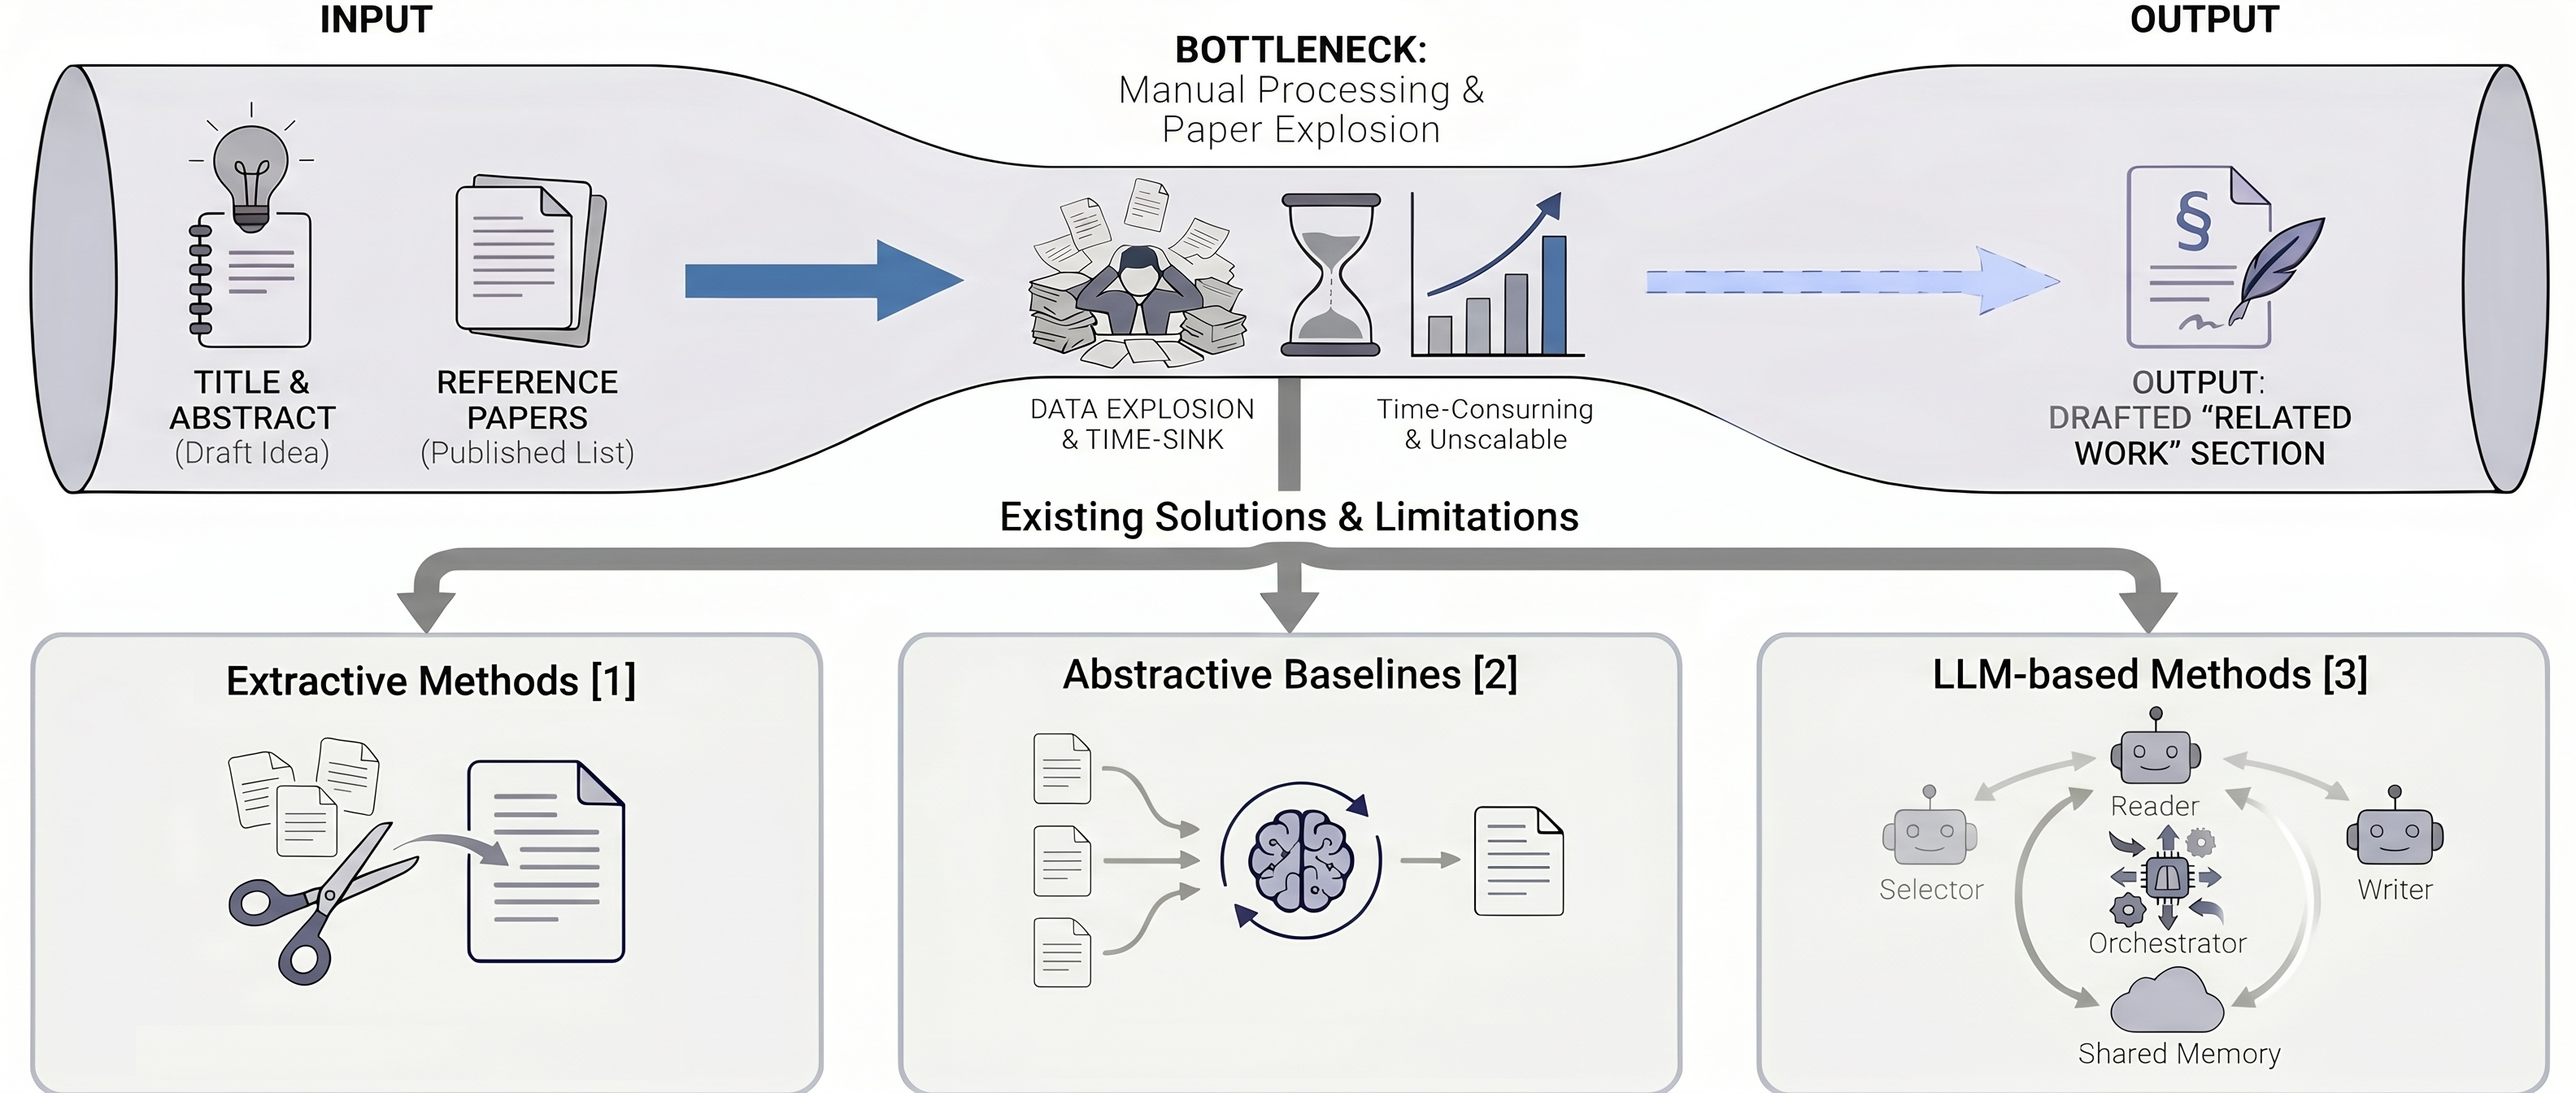
\includegraphics[width=\textwidth,height=0.65\textheight,keepaspectratio]{diagram_final.jpg}
    \end{center}

    \vfill
    \slidesources{%
        \parbox{\textwidth}{%
            \fontsize{5pt}{6pt}\selectfont\color{gray}%
            \hyperlink{refs}{\cite{hoang2010towards} \fullcite{hoang2010towards}}\\[1pt]%
            \hyperlink{refs}{\cite{xiao2022primera} \fullcite{xiao2022primera}}\\[1pt]%
            \hyperlink{refs}{\cite{liu2025select} \fullcite{liu2025select}}%
        }%
    }
\end{frame}
    \section{Related Work}
    \begin{frame}[t]
    \vspace{-8mm}
    \frametitle{Proposed Framework}
    \vspace{2mm}

    \begin{figure}
        \centering
        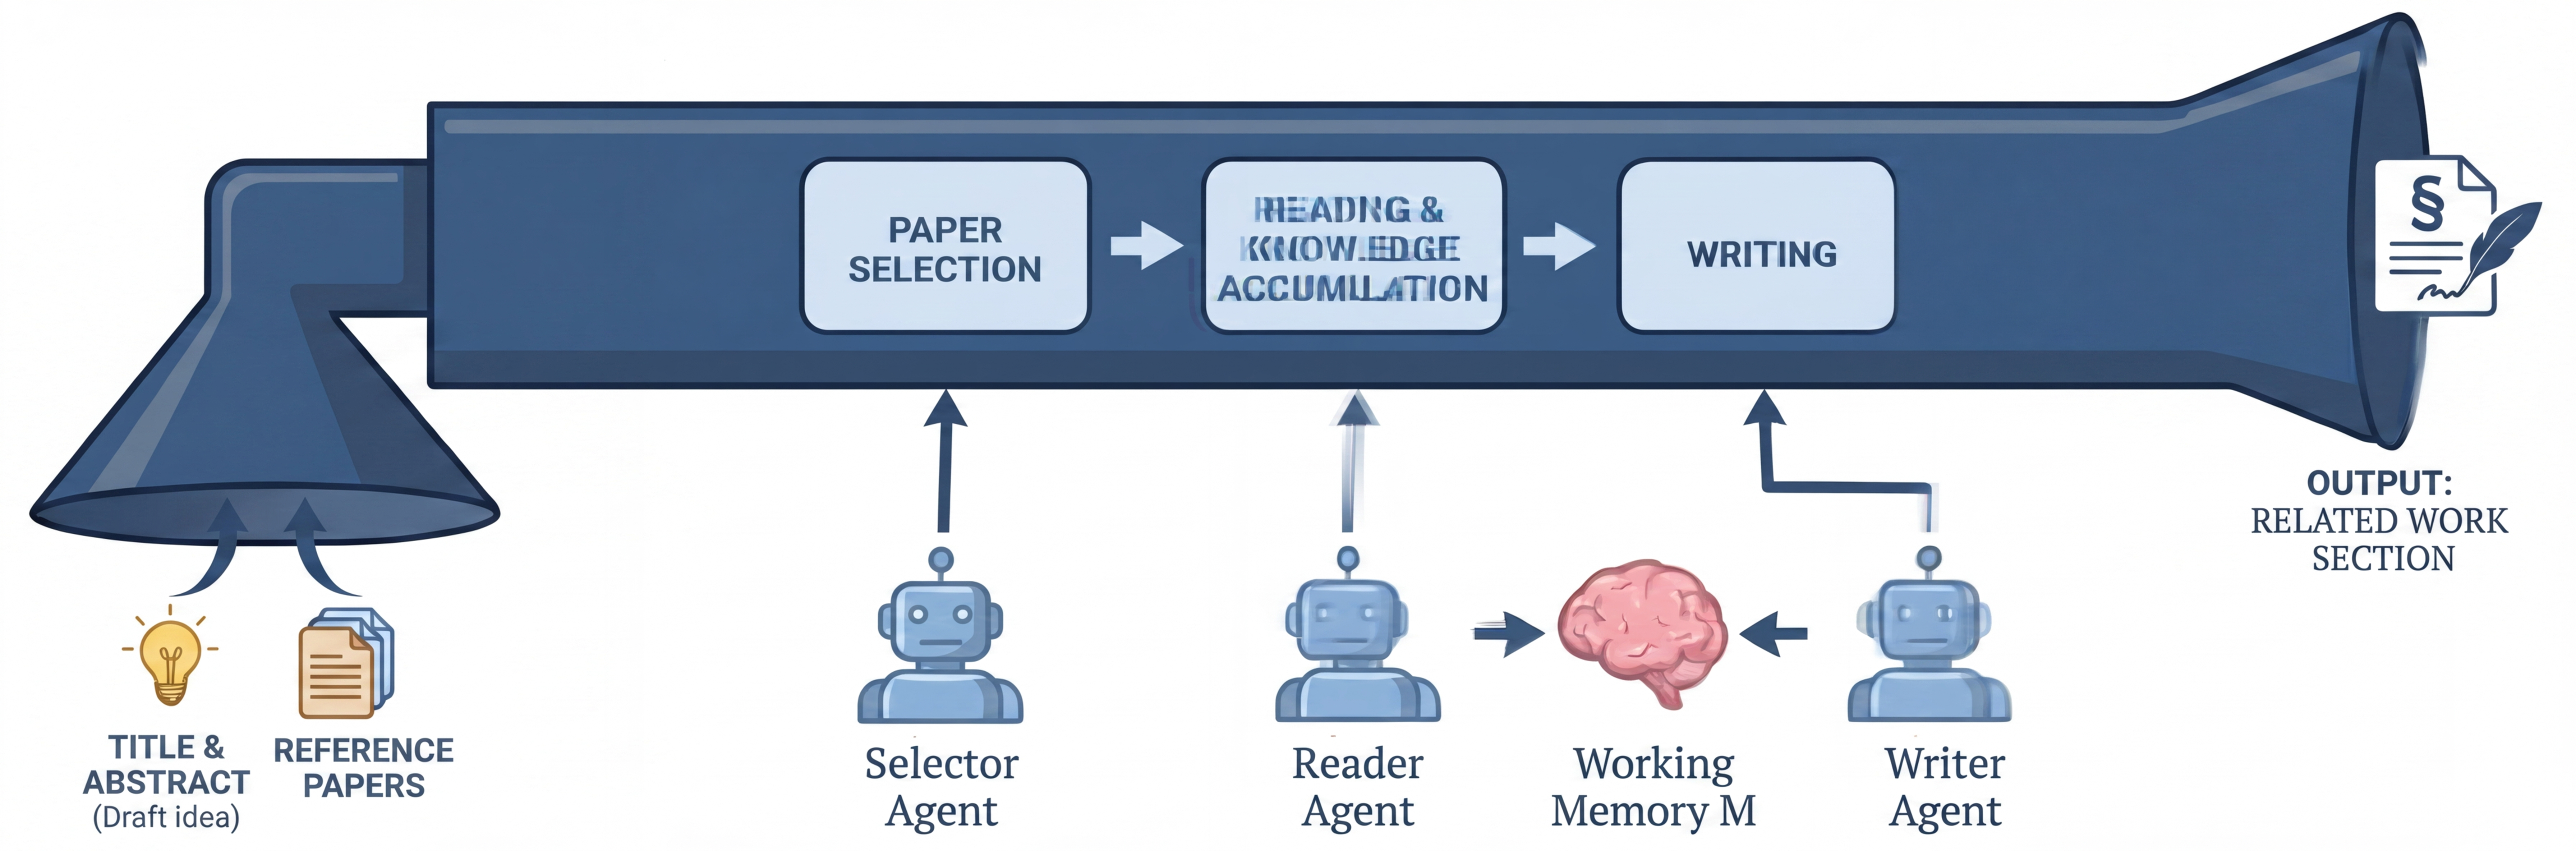
\includegraphics[width=0.7\textwidth, height=2.5cm, keepaspectratio]{pipeline.jpg}
        \caption{Prior work leveraging LLM-based method.}
    \end{figure}

    \vspace{-4mm}

    \begin{figure}
        \centering
        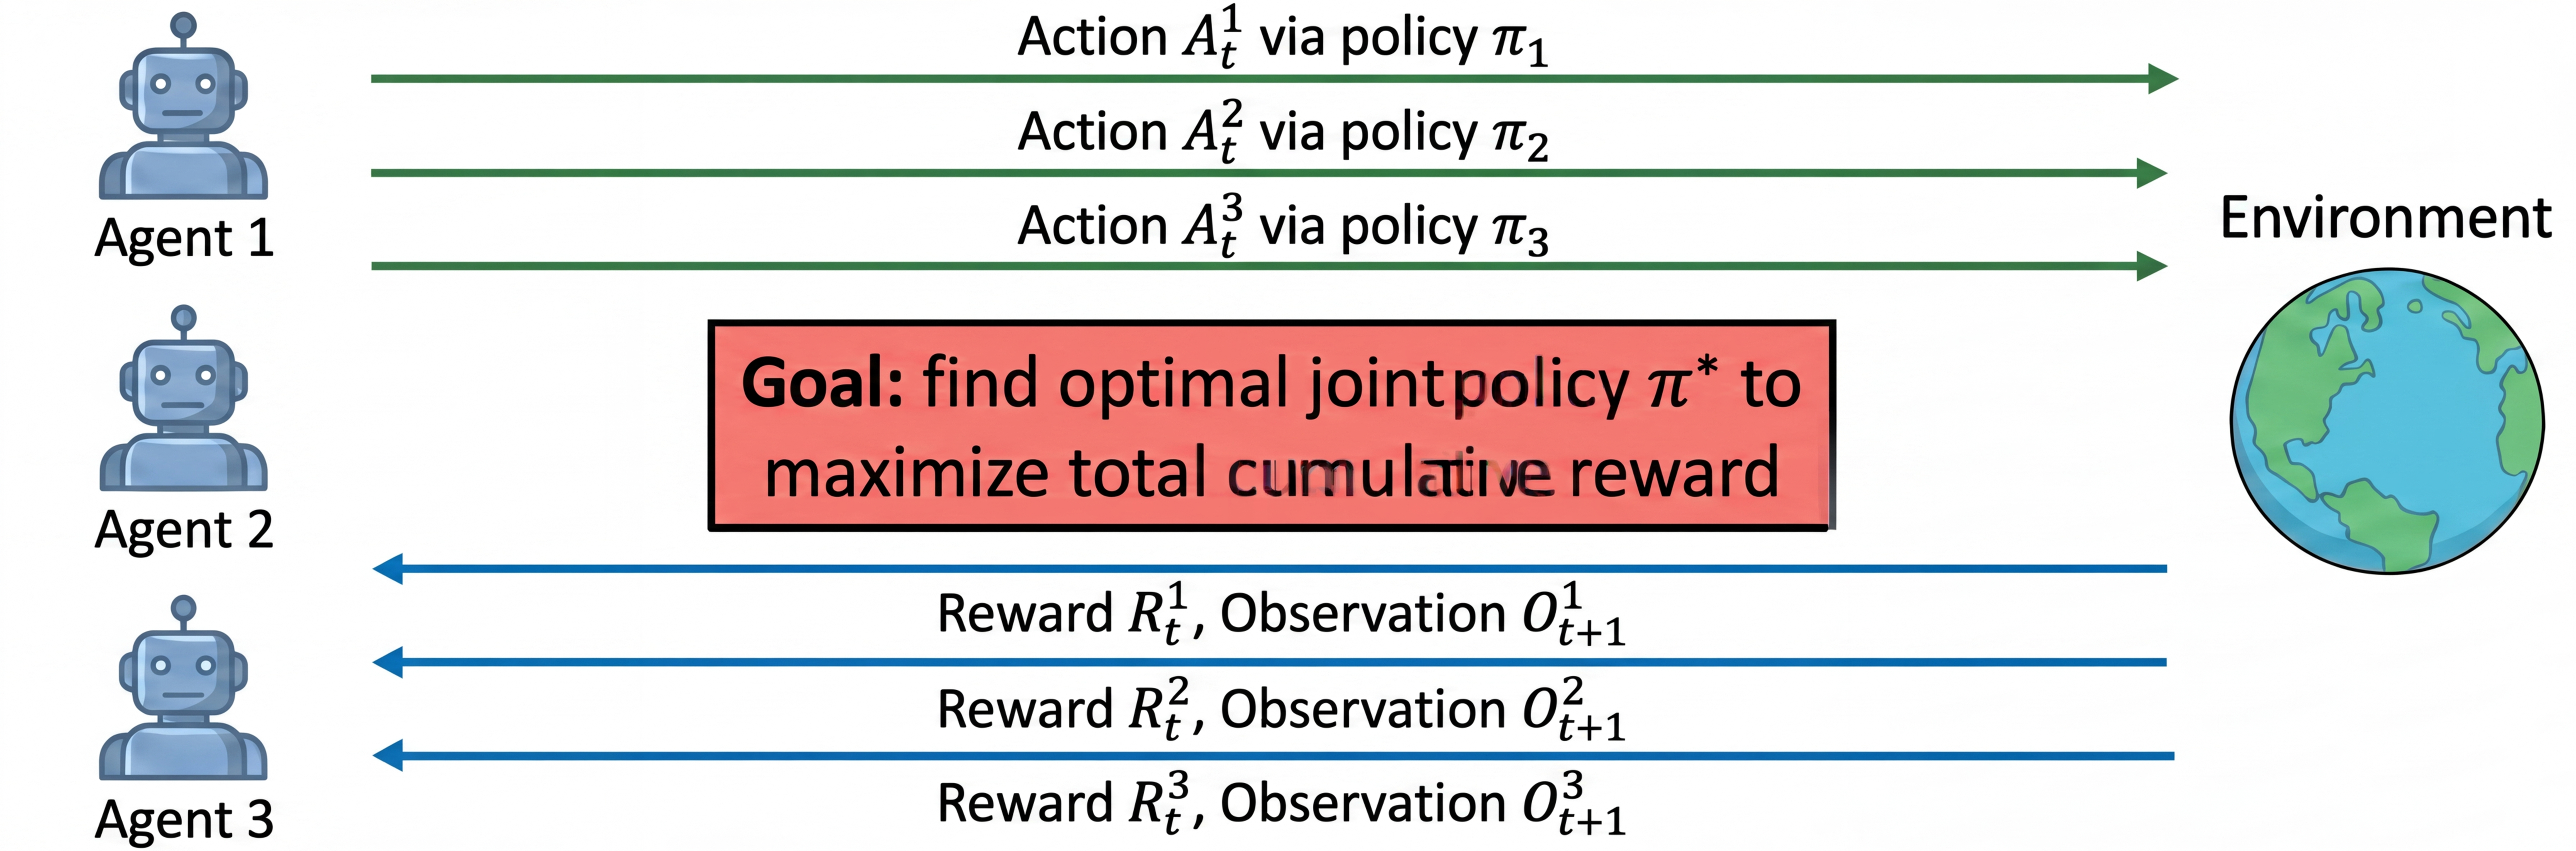
\includegraphics[width=0.7\textwidth, height=2.5cm, keepaspectratio]{marl.jpg}
        \caption{A Collaborative Multi-agent Reinforcement Learning-Based Framework (CREW).}
    \end{figure}
\end{frame}


    \section{Methodology}
    
\begin{frame}[t]
    \frametitle{Architecture}
    \vspace{-2mm}
    
    \begin{figure}
        \centering
        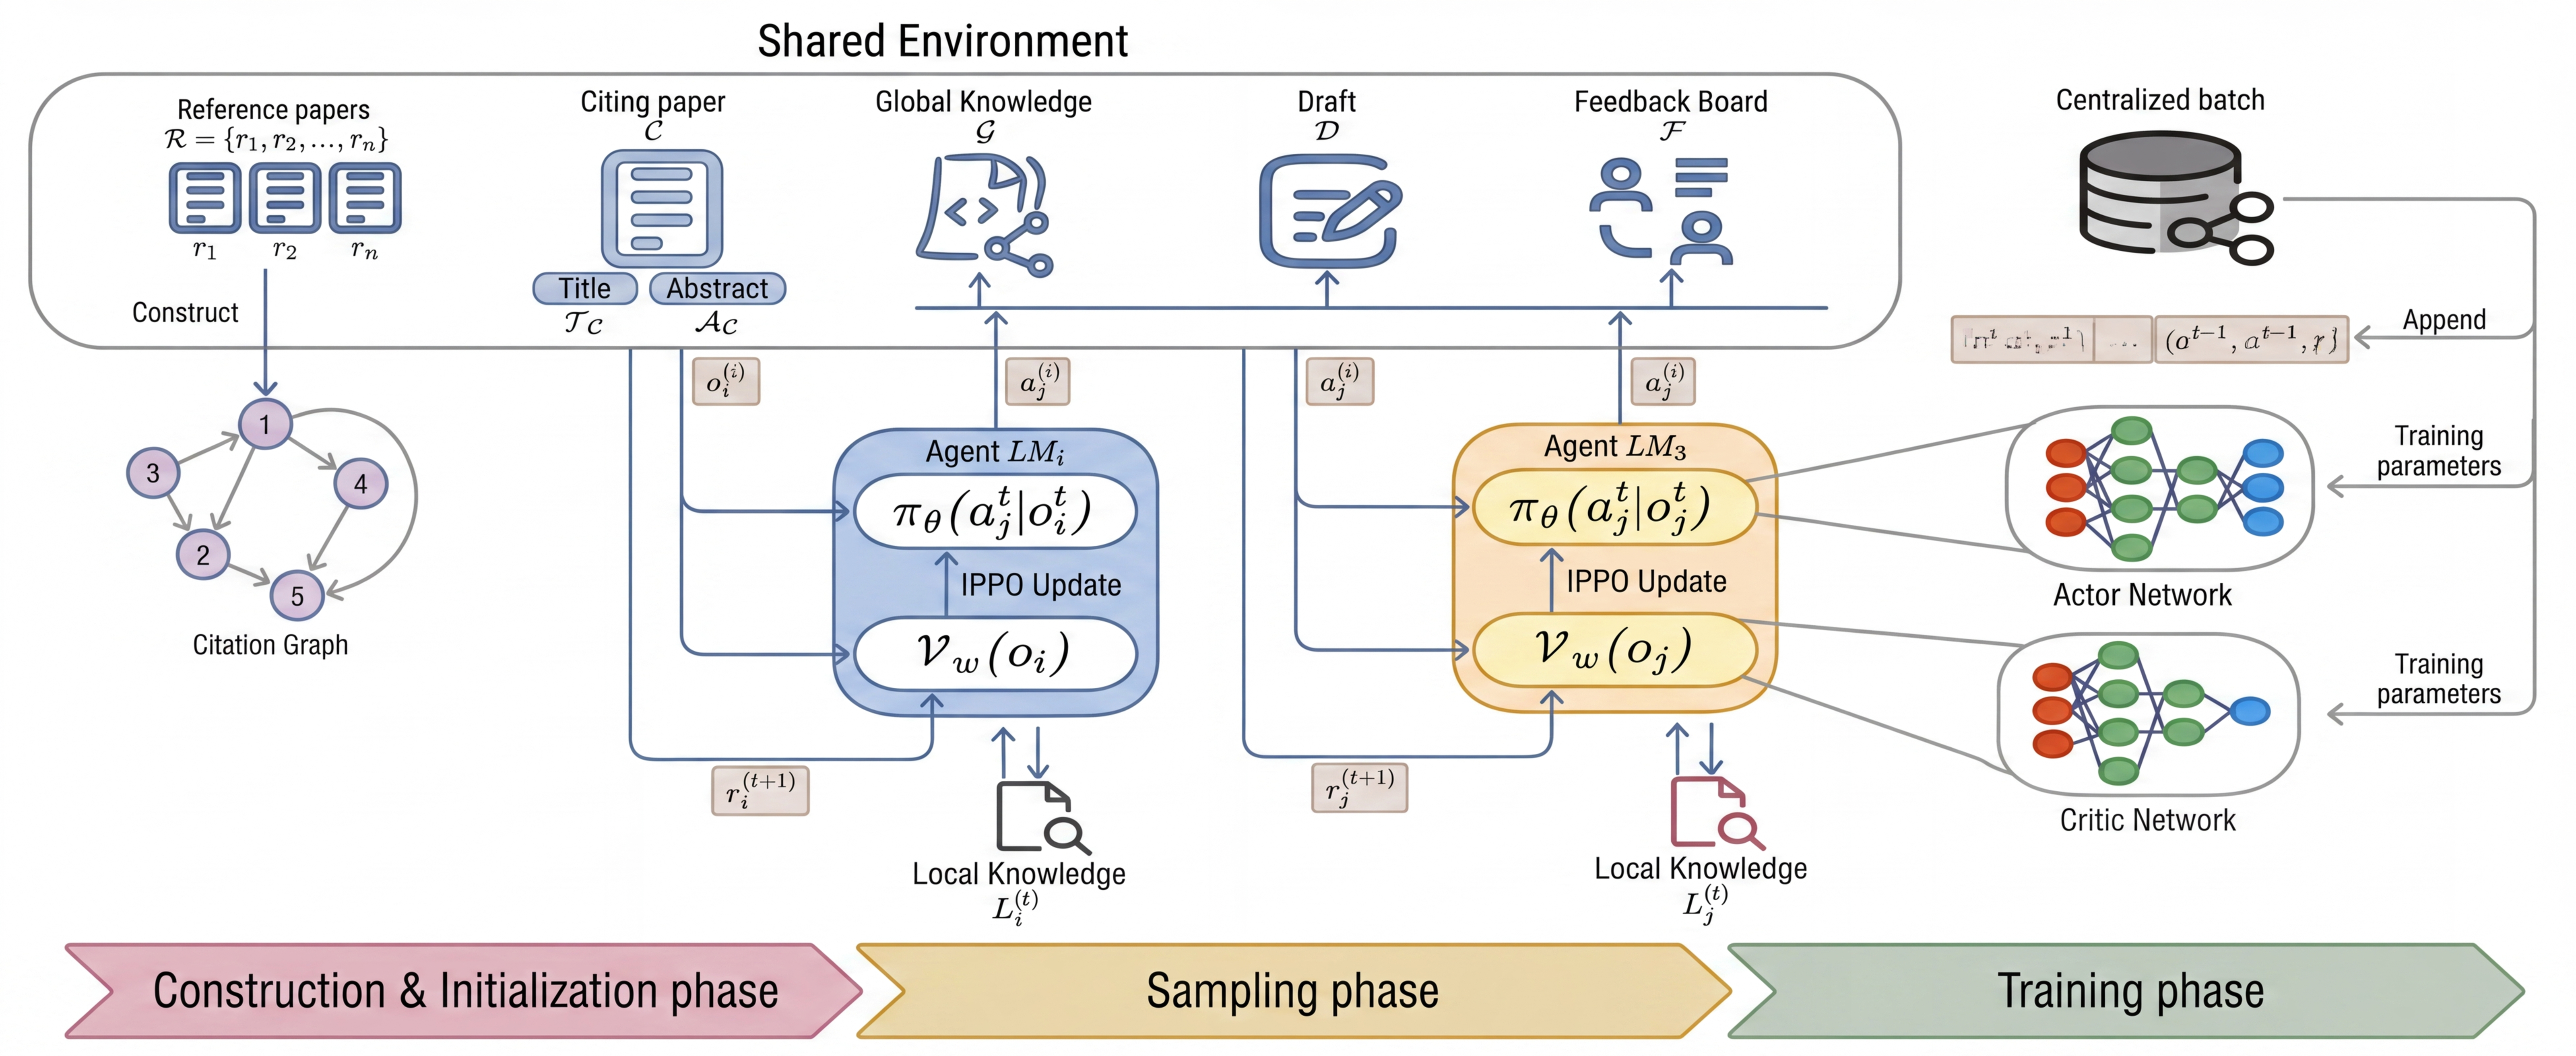
\includegraphics[height=0.75\textheight, keepaspectratio]{architechture_super_final.jpg}
        \caption{Proposed system architecture overview.}
    \end{figure}
\end{frame}

    \section{Performance Evaluation}
    \setbeamertemplate{caption label separator}{. }
\setbeamerfont{caption}{size=\tiny}

\begin{frame}[t]
\vspace{1mm} % Slightly down from the top red line
\frametitle{Experimental Setup and Results}

% SECTION 1: Experimental Setup
\textcolor{red}{\footnotesize$\blacktriangleright$} \textbf{\footnotesize Experimental Setup}
\begin{itemize}[leftmargin=1.5em, itemsep=0.1em, topsep=0.1em, label=\textcolor{blue!70!black}{\tiny$\bullet$}]
    \footnotesize
    \item Environment: Python 3.10, NVIDIA A100 GPU (Train \& Infer: Qwen-32B-Instruct).
    \item Dataset: OARelatedWork \cite{docekal2024oarelatedwork}.
    \item Metrics: LLM-as-a-Judge (inc. Coverage, Logic, Relevance) \cite{liu2025select}.
    \item Baselines: PRIMERA \cite{xiao2022primera}, GPT-4o, Select-RW \cite{liu2025select}.
\end{itemize}

\vspace{0mm} % Tightened spacing

% SECTION 2: Results
\textcolor{red}{\footnotesize$\blacktriangleright$} \textbf{\footnotesize Results}
\vspace{-6mm} % Pull the entire table block up

\begin{columns}[T]
    % LEFT COLUMN: Table 1 (Narrower)
    \begin{column}{0.42\textwidth}
        \begin{table}[H]
            \caption{Effectiveness}
            \centering
            \tiny
            \vspace{-1.5mm} % Close gap to caption
            \begin{tabular}{l c c c c c}
            \toprule
            \textbf{Model} & \textbf{Cov.} & \textbf{Log.} & \textbf{Rel.} & \textbf{Avg.} & \textbf{Tok.} \\
            \midrule
            PRIMERA & 2.48 & 2.71 & 3.02 & 2.64 & 186K \\
            GPT-4o & 3.18 & 4.08 & 3.96 & 3.36 & 2.1K \\
            Select-RW & 3.36 & 4.21 & 4.18 & 3.53 & 186K \\
            \midrule
            \textbf{CREW} & \textbf{3.62} & \textbf{4.39} & \textbf{4.31} & \textbf{3.77} & \textbf{153K} \\
            \bottomrule
            \end{tabular}
        \end{table}
    \end{column}
    
    % RIGHT COLUMN: Table 2 (Wider for delta values)
    \begin{column}{0.57\textwidth}
        \begin{table}[H]
            \caption{Ablation Study}
            \centering
            \tiny
            \vspace{-1.5mm} % Close gap to caption
            \begin{tabular}{l c c c c c}
            \toprule
            \textbf{Config} & \textbf{Cov.} & \textbf{Log.} & \textbf{Rel.} & \textbf{Avg.} & \textbf{Tok.} \\
            \midrule
            w/o Draft & 3.41 {\color{red}\tiny(-.21)} & 4.02 {\color{red}\tiny(-.37)} & 4.10 {\color{red}\tiny(-.21)} & 3.50 {\color{red}\tiny(-.27)} & 150K \\
            w/o Crit. & 3.35 {\color{red}\tiny(-.27)} & 4.08 {\color{red}\tiny(-.31)} & 4.02 {\color{red}\tiny(-.29)} & 3.42 {\color{red}\tiny(-.35)} & 143K \\
            w/o BB. & 3.29 {\color{red}\tiny(-.33)} & 3.95 {\color{red}\tiny(-.44)} & 3.98 {\color{red}\tiny(-.33)} & 3.35 {\color{red}\tiny(-.42)} & 160K \\
            \midrule
            \textbf{CREW} & \textbf{3.62} & \textbf{4.39} & \textbf{4.31} & \textbf{3.77} & \textbf{153K} \\
            \bottomrule
            \end{tabular}
        \end{table}
    \end{column}
\end{columns}

\vfill
\slidesources{%
    \parbox{\textwidth}{%
        \fontsize{5pt}{6pt}\selectfont\color{gray}%
        \hyperlink{refs}{\cite{docekal2024oarelatedwork} \fullcite{docekal2024oarelatedwork}}\\[1pt]%
        \hyperlink{refs}{\cite{xiao2022primera} \fullcite{xiao2022primera}}\\[1pt]%
        \hyperlink{refs}{\cite{liu2025select} \fullcite{liu2025select}}%
    }%
}
\end{frame}
    \begin{frame}[t]
\frametitle{Case Study}
\vspace{2mm}

% Paper Title & Abstract Box
\begin{beamercolorbox}[wd=\textwidth, sep=3pt, rounded=true]{block title}
    \scriptsize \textbf{Target Paper:} Robust Non-Rigid Registration of 2D and 3D Graphs
\end{beamercolorbox}
\begin{beamercolorbox}[wd=\textwidth, sep=4pt, rounded=true]{block body}
    \tiny \textbf{Abstract:} We present a new approach to matching graphs in $\mathbb{R}^2$ or $\mathbb{R}^3$. Our method handles partial matches and non-linear deformations using Gaussian Processes, without requiring appearance features or initial alignment... [...]
\end{beamercolorbox}

\vspace{-1mm}
\begin{columns}[T, onlytextwidth]
    % Select-RW (Baseline)
    \begin{column}{0.48\textwidth}
        \centering
        {\scriptsize \color{hustprimary} \textbf{Baseline: Select-RW \cite{liu2025select}}} \par
        \vspace{1mm}
        \begin{minipage}[t][4.2cm]{\textwidth}
            \tiny \raggedright
            \redhl{Advanced techniques have emerged to overcome these} \redhl{limitations.} One notable approach is the SoftPosit algorithm. \redhl{Despite its effectiveness, the SoftPosit algorithm} \redhl{can still fail} in the presence of clutter or occlusions \redhl{\textbf{[3755653]}}.
            \vspace{1mm} \par
            To address these limitations, a recent paper \redhl{proposes an} \redhl{innovative solution} by integrating a GMM to refine pose priors \redhl{\textbf{[3755653]}}. \redhl{This method progressively refines} the pose estimates by hypothesizing correspondences. \redhl{By reducing matches and exploring the pose space} \redhl{more thoroughly,} this approach enhances the robustness and efficiency \redhl{\textbf{[3755653]}}.
        \end{minipage}
    \end{column}

    % CREW (Ours)
    \begin{column}{0.48\textwidth}
        \centering
        {\scriptsize \color{hustprimary} \textbf{Ours: CREW}} \par
        \vspace{1mm}
        \begin{minipage}[t][4.2cm]{\textwidth}
            \tiny \raggedright
            \greenhl{While [28637] and [27485] focus on geometric and} \greenhl{appearance priors,} other methodologies such as spectral methods and deep learning have also been explored. \greenhl{Spectral methods, which leverage the eigenvalues and} \greenhl{eigenvectors of graph Laplacians, offer a powerful tool} for graph matching by capturing the intrinsic structure. \greenhl{These methods are particularly useful for regular} \greenhl{structures where dominant eigenvalues are present.} However, they struggle with nonlinear deformations, which are \greenhl{better handled by geometric approaches in [28637].}
        \end{minipage}
    \end{column}
\end{columns}

\vfill
\slidesources{%
    \parbox{\textwidth}{%
        \fontsize{5pt}{6pt}\selectfont\color{gray}%
        \hyperlink{refs}{\cite{liu2025select} \fullcite{liu2025select}}%
    }%
}
\end{frame}

    \section{Conclusions and Future Work}
    \begin{frame}[t]
\vspace{-2mm}
\frametitle{Conclusions and Future Work}
\footnotesize

\vspace{0.4cm}
\textcolor{red}{\small$\blacktriangleright$} \textbf{Conclusions}
\begin{itemize}[leftmargin=2em, itemsep=0.3cm, topsep=0.1cm, label=\textcolor{blue!70!black}{\tiny$\bullet$}]
    \item \textbf{Collaborative Framework:} Proposed CREW, a MARL-based system for automated related work summarization.
    \item \textbf{Empirical Success:} Improved coverage, relevance, and logic through dynamic agent coordination.
\end{itemize}

\vspace{0.5cm}
\textcolor{red}{\small$\blacktriangleright$} \textbf{Future Work}
\begin{itemize}[leftmargin=2em, itemsep=0.3cm, topsep=0.1cm, label=\textcolor{blue!70!black}{\tiny$\bullet$}]
    \item \textbf{System Expansion:} Integrate external database crawling and dynamic online document graphs.
\end{itemize}

\vfill
\centering
\textcolor{red}{\Large\textbf{THANK YOU FOR LISTENING!}}
\vspace{4mm}

\end{frame}
    
    \useStyleLogoOnly 
    \setbeamertemplate{bibliography item}[text]
    
    \begin{frame}[allowframebreaks, label=refs]{References}
        \tiny
        \printbibliography[heading=none]
    \end{frame}

\end{document}